\graphicspath{ {imgs/} }
\documentclass[main.tex]{subfiles}
\begin{document}
\chapter{Methods}\label{chap:methods}
The following sections highlight the used methods and give a rough overview about the used tools. First the used environment of software tools is described. Then the theoretical concept of a Convolutional Neural Network is explained and how it was trained on the available resources. A more extensive explanation to the different software packages and computational resources can be found in the appendix~\ref{app:software}.

\section{Software Packages}
Writing a program for solving the task of nodule detection with neural networks makes the use of certain frameworks necessary. Using Python as a versatile programming language allowed for writing code for all aspects of the project: from data preprocessing and training the network to analyzing the results. The language narrows down the number of frameworks available for training neural networks. For this thesis Tensorflow (\ref{appendix:tf}) was chosen since it is at the moment the most active framework (in the sense of implementation  Figure~\ref{fig:frameworks}). Other frameworks like Cafe, Theano and Keras would have been valid choices as well. The Sun Grid Engine of the institute is used for automated execution on several machines (see ~\ref{appendix:oge} for details) and was used for training the model.

\begin{figure}
\begin{center}
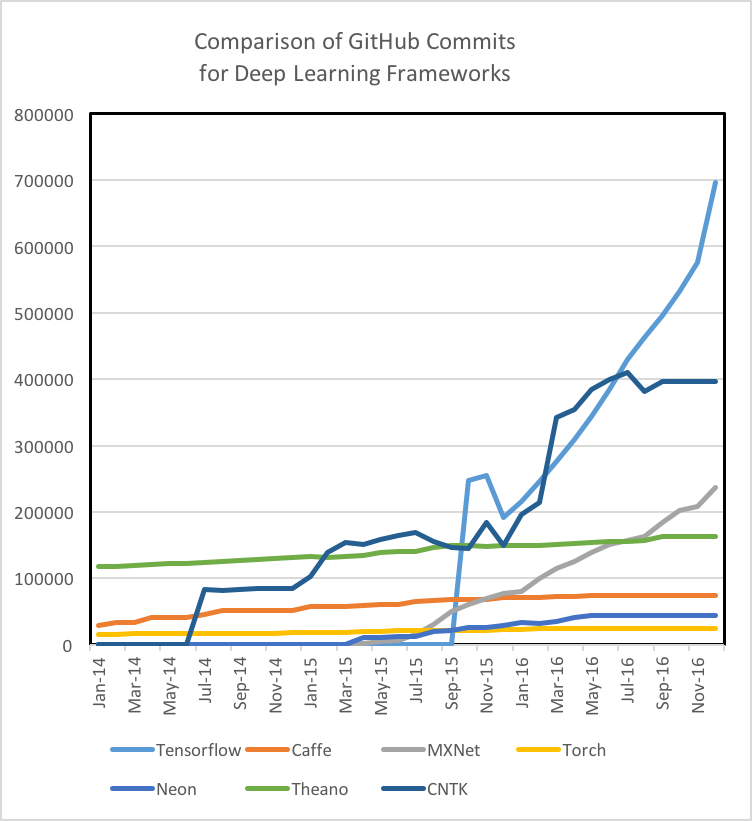
\includegraphics[scale=0.7]{deeplearning_frameworks.png}
\end{center}
\caption{Number of commits for the different deep learning frameworks. This figure is taken from Shapiro \cite{shapiro2017}.}
\label{fig:frameworks}
\end{figure}



\section{Convolutional Neural Network}
In this thesis a 3D Convolutional Neural Network (CNN) is used to classify the CT slices. The main motivation to use a 3D CNN in the case of nodule detection are the morphological features of the nodules that could not be fully utilized by a convolution that is only applied to 2D sections of the nodule. A CNN is similar to other artificial neural networks (ANNs) in the sense that it only uses forward connections, has an input and output layer and an arbitrary number of hidden layers in between. The hidden layers in a convolutional network are either convolutional or pooling layers which are in the end followed by one or more dense layers that perform the classification. Each of those layers is described in more detail in the following sections.

\subsection{Convolutional Layer}\label{ss:convlayer}
The convolutional layer consists of $1..n$ kernels that are represented through shared weights that compared to classic convolution in computer vision do not \emph{slide} across the input but are duplicated across the image in the defined distance (called stride). For this CNN $3$ convolutional layers were used with $32$, $16$ and $16$ kernels each. The convolution takes place in 3D which means that the filter kernels are also 3 dimensional and the stride is as well defined in all 3 directions of the input image $(x,y,z)$. The kernel size was chosen to be $(3x3x3)$ in accordance with Huang et al.'s\cite{huang2017lung} implementation for nodule classification. 

\begin{figure}
\begin{center}
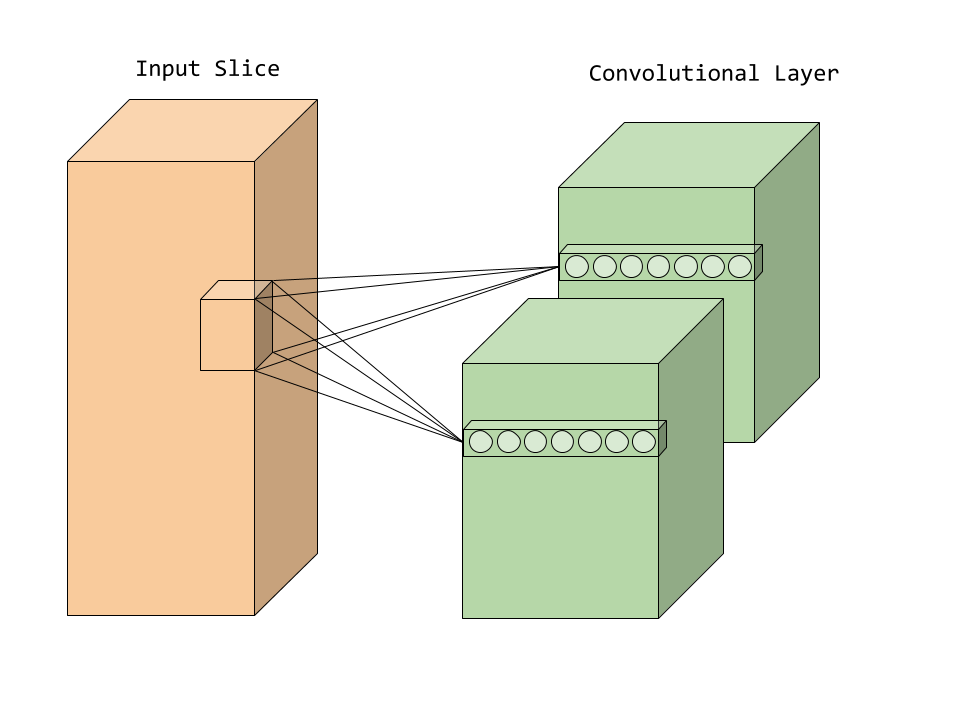
\includegraphics[scale=0.3]{conv_layer.png}
\end{center}
\caption{Structure of a convolutional layer. In image analysis the third dimension may encode the color informational, but in the example of Lung CT data it encodes additional spatial information. The figure shows two separate kernels that have shared weights for each kernel position in the input.}
\label{fig:conv_layer}
\end{figure}

As the layers of convolution stack the extracted features from the first layer are combined to more complex shapes. The layers contain also a batchnormalization step as described in \cite{ioffe2015batch} that was implemented in the Tensorflow layers class. Batchnormalization is scaling the activation of the layer to become normally distributed in each dimension of the features, but has additional parameters that can be learned to shift and scale these values again. This should bring several advantages like: reducing the dependence of the initialization method and allowing for higher learning rates. The batchnormalization is followed by a max pooling layer which is applying a max-filter of size $(2,2,2)$ to the normalized activations.


\subsection{Dense Layers}
The activations from the last convolutional layer are flattened into a $(1 \times n)$ vector and fed to the neurons of the fully connected layer. The network has two dense layers with $64$ neurons each. The activation function of the rectified linear unit is a simple maximum of the weighted inputs. The combined complete structure of the network can be seen in Figure~\ref{fig:net_struct}.

\begin{figure}
\begin{center}
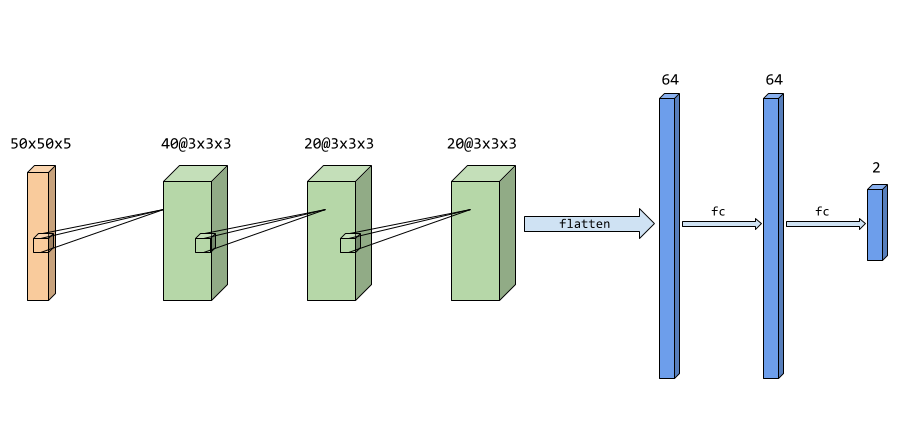
\includegraphics[scale=0.5]{net_struct.png}
\end{center}
\caption{Architecture of the neural network. Each of the convolutional layers is composed of a 3D convolution layer with the respective filter size followed by a batchnormalization and a pooling layer. The pool size is $(2,2,2)$ with a stride of $(1,1,1)$. The structure of the neural network resembles closely the one described by Huang~\cite{huang2017lung}.}
\label{fig:net_struct}
\end{figure}


\section{Training}
The input to the network are the slices that have been the result of the before described preprocessing and are fed to the network in batches. They are augmented by randomly flipping them in x and y plane (examples can be seen in \ref{fig:input}). The augmentation is applied to make the learned classification more robust against distortions in the input. It makes sense in this specific scenario since the nodules are growing in different shapes and locations in the lung and flipping them is not producing an impossible input to the network.

\begin{figure}
\begin{center}
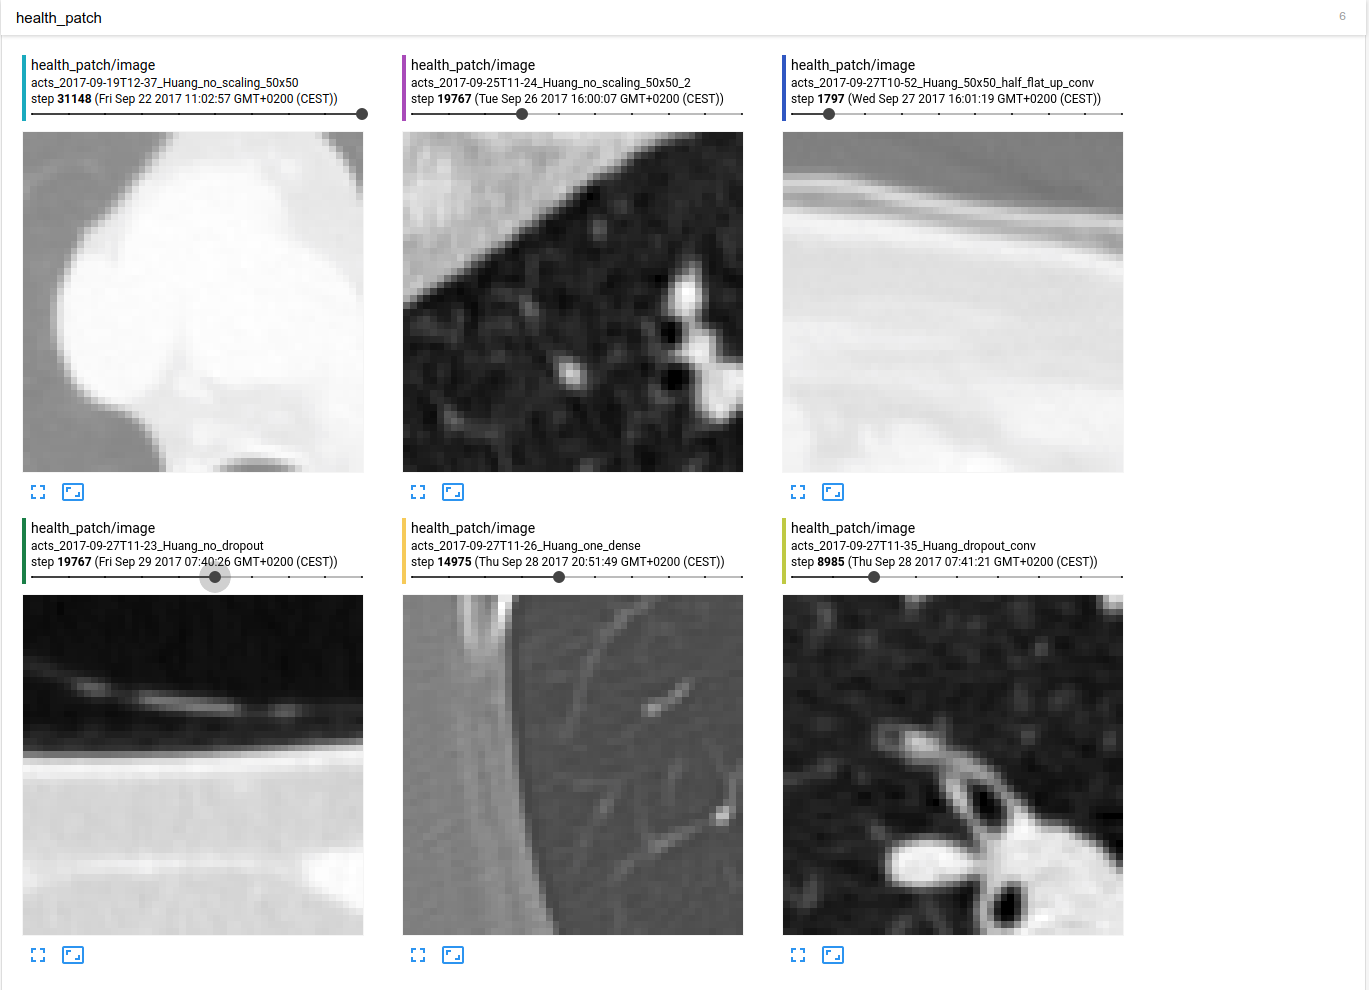
\includegraphics[scale=0.25]{patches-health.png}
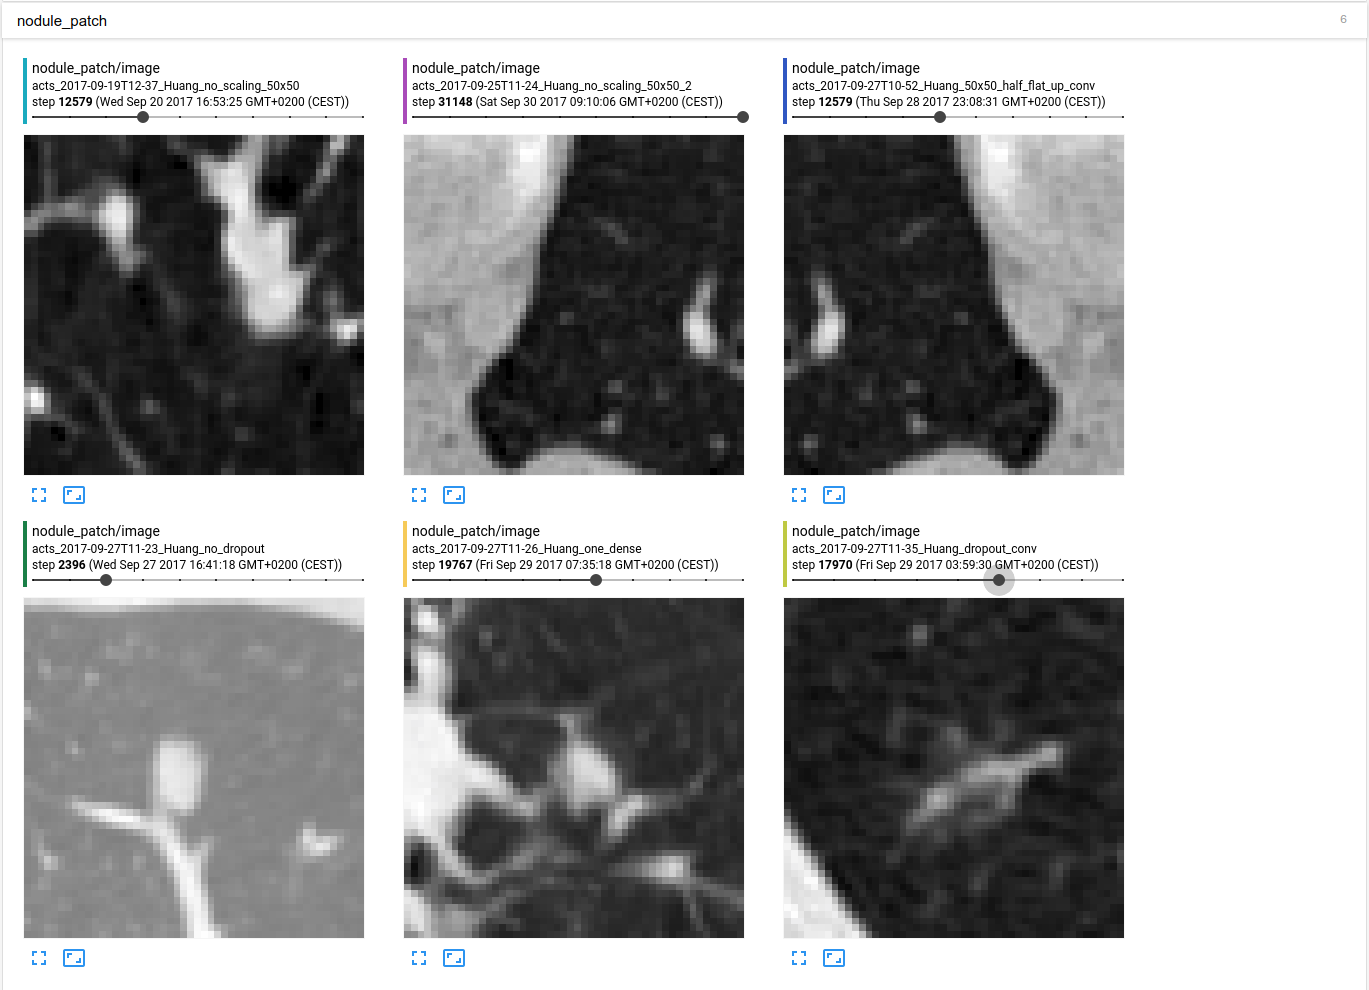
\includegraphics[scale=0.25]{patches-nodule.png}
\end{center}
\caption{Input data for the cases of healthy and nodule patches. The image is taken from Tensorboard and shows in the case of nodules the random permutation of the input data.}
\label{fig:input}
\end{figure}

Regularization methods used for this network include batchnormalization and dropout. Batchnormalizaton is in TensorFlow implemented as described by Ioffe and Szegedy~\cite{ioffe2015batch} and has been described already in section~\ref{ss:convlayer}. Dropout is another regularization method that was used in this thesis. It basically means that during training random neurons of the network are dropped - training effectively several models at once, as discovered by Srivastava et al.~\cite{srivastava2014dropout}, which should increase the overall performance of the network. During training no improved performance could be observed when applying dropout throughout the whole network. It was rather harmful if applied to the convolutional layers. The final model uses dropout only in the fully connected  layers.


\end{document}
